\documentclass[9pt,a4paper]{article}
\usepackage[frenchb]{babel}
\usepackage[utf8]{inputenc}
\usepackage[T1]{fontenc}
\usepackage{lmodern}
\usepackage{amsmath}
\usepackage{tikz}
\usepackage{cite}
\usepackage{hyperref}
\usepackage{fancyvrb}
\usepackage{bm}
\usepackage{pxfonts}


% Alter some LaTeX defaults for better treatment of figures:
% See p.105 of "TeX Unbound" for suggested values.
% See pp. 199-200 of Lamport's "LaTeX" book for details.
% General parameters, for ALL pages:
\renewcommand{\topfraction}{0.9}  % max fraction of floats at top
\renewcommand{\bottomfraction}{0.8} % max fraction of floats at bottom
% Parameters for TEXT pages (not float pages):
\setcounter{topnumber}{2}
\setcounter{bottomnumber}{2}
\setcounter{totalnumber}{4}     % 2 may work better
\setcounter{dbltopnumber}{2}    % for 2-column pages
\renewcommand{\dbltopfraction}{0.9} % fit big float above 2-col. text
\renewcommand{\textfraction}{0.07}  % allow minimal text w. figs
% Parameters for FLOAT pages (not text pages):
\renewcommand{\floatpagefraction}{0.7}  % require fuller float pages
% N.B.: floatpagefraction MUST be less than topfraction !!
\renewcommand{\dblfloatpagefraction}{0.7} % require fuller float pages

% remember to use [htp] or [htpb] for placement


\newcommand{\FIXME}{\textcolor{red}{FIXME}}
%\newcommand{\TODO}[1]{(\textcolor{red}{TODO} #1)}
\newcommand{\TODO}[1]{}
\newcommand{\LANG}{Heptagon}

\newcommand{\bold}[1]{\textbf{#1}}
\newcommand{\p}[0]{\; \vert \;}
\newcommand{\rst}[1]{Rst(#1)}
\newcommand{\rstnd}[1]{RstNode(#1)}
% \newcommand{\rst}[1]{\llbracket #1 \rrbracket^{rst}}
\newcommand{\tvh}[2]{\llbracket #2 \rrbracket^{vhdl\ #1}}
\newcommand{\guardb}[1]{\llbracket #1 \rrbracket^{guard}}
\newcommand{\guard}[2]{\mbox{if } \guardb{#1} \mbox{ then } #2 \mbox{ else }
  \emptyset}
\newcommand{\mybox}[1]{\mbox{\tt{#1}}}
\newcommand{\bl}[0]{\hspace{0.45cm}}
\newcommand{\ind}[0]{\hspace{0.5cm}}
\newcommand{\Cons}[0]{\; \mathbf{::} \;}

%% Syntaxe MiniLS

\newcommand{\Node}[4]{\mybox{node} \; f(#1) = #2 \; \mybox{with var} \
  #3 \; \mybox{in} \; #4}
\newcommand{\Op}[2]{\mybox{\bf{op}}(#1,\dots,#2)}
\newcommand{\Fby}[2]{#1 \, \mybox{fby}^{ck} \, #2}
\newcommand{\Pre}[1]{\mybox{pre}^{ck} \, #1}
\newcommand{\Every}[4]{#1^{ck}(#2,\dots,#3) \, \mybox{every} \, #4}
\newcommand{\App}[2]{#1^{ck}(#2)}
\newcommand{\If}[3]{\mybox{if} \; #1 \; \mybox{then} \; #2 \; \mybox{else} \; #3}
\newcommand{\When}[3]{#1 \; \mybox{when} \; #2(#3)}
\newcommand{\Merge}[5]{\mybox{merge} \; #1 \; (#2 \Rightarrow #3) \; \dots \; \
  (#4 \Rightarrow #5)}
\newcommand{\Base}[0]{\mybox{base}}
\newcommand{\On}[3]{#1 \mybox{ on } #2 (#3)}
\newcommand{\Map}[3]{\mathtt{map} \; #1 n (#2,\dots,#3)}
\newcommand{\Fold}[3]{\mathtt{fold} \; #1 n (#2,\dots,#3)}
\newcommand{\Mapfold}[3]{\mathtt{mapfold} \; #1 n (#2,\dots,#3)}

%% Syntaxe VHDL

\newcommand{\Component}[6]{\mybox{component} \; #1 \; \mybox{port} \; #2 \; \
  \mybox{with} \; \mybox{sig} \; #3 \; \mybox{and} \; \mybox{var} \; #4 \; \\
  \mybox{and} \; \mybox{subcomponents} \; #5 \; \mybox{in} \; #6}

\newcommand{\Assign}[2]{#1 \Leftarrow #2}
\newcommand{\Affect}[2]{#1 \coloneqq #2}
\newcommand{\Case}[5]{\mybox{case} \; #1 \; \mybox{of} \; (#2 \Rightarrow #3) \
  \dots (#4 \Rightarrow #5)}

\title{\LANG{} vers VHDL}
\author{Adrien Guatto et Marc Pouzet}


\makeatletter
\def\PY@reset{\let\PY@it=\relax \let\PY@bf=\relax%
    \let\PY@ul=\relax \let\PY@tc=\relax%
    \let\PY@bc=\relax \let\PY@ff=\relax}
\def\PY@tok#1{\csname PY@tok@#1\endcsname}
\def\PY@toks#1+{\ifx\relax#1\empty\else%
    \PY@tok{#1}\expandafter\PY@toks\fi}
\def\PY@do#1{\PY@bc{\PY@tc{\PY@ul{%
    \PY@it{\PY@bf{\PY@ff{#1}}}}}}}
\def\PY#1#2{\PY@reset\PY@toks#1+\relax+\PY@do{#2}}

\def\PY@tok@gd{\def\PY@tc##1{\textcolor[rgb]{0.63,0.00,0.00}{##1}}}
\def\PY@tok@gu{\let\PY@bf=\textbf\def\PY@tc##1{\textcolor[rgb]{0.50,0.00,0.50}{##1}}}
\def\PY@tok@gt{\def\PY@tc##1{\textcolor[rgb]{0.00,0.25,0.82}{##1}}}
\def\PY@tok@gs{\let\PY@bf=\textbf}
\def\PY@tok@gr{\def\PY@tc##1{\textcolor[rgb]{1.00,0.00,0.00}{##1}}}
\def\PY@tok@cm{\def\PY@tc##1{\textcolor[rgb]{0.50,0.50,0.50}{##1}}}
\def\PY@tok@vg{\let\PY@bf=\textbf\def\PY@tc##1{\textcolor[rgb]{0.82,0.44,0.00}{##1}}}
\def\PY@tok@m{\let\PY@bf=\textbf\def\PY@tc##1{\textcolor[rgb]{0.38,0.00,0.88}{##1}}}
\def\PY@tok@mh{\let\PY@bf=\textbf\def\PY@tc##1{\textcolor[rgb]{0.00,0.31,0.50}{##1}}}
\def\PY@tok@cs{\let\PY@bf=\textbf\def\PY@tc##1{\textcolor[rgb]{0.80,0.00,0.00}{##1}}}
\def\PY@tok@ge{\let\PY@it=\textit}
\def\PY@tok@vc{\def\PY@tc##1{\textcolor[rgb]{0.19,0.38,0.56}{##1}}}
\def\PY@tok@il{\let\PY@bf=\textbf\def\PY@tc##1{\textcolor[rgb]{0.00,0.00,0.82}{##1}}}
\def\PY@tok@go{\def\PY@tc##1{\textcolor[rgb]{0.50,0.50,0.50}{##1}}}
\def\PY@tok@cp{\def\PY@tc##1{\textcolor[rgb]{0.31,0.44,0.56}{##1}}}
\def\PY@tok@gi{\def\PY@tc##1{\textcolor[rgb]{0.00,0.63,0.00}{##1}}}
\def\PY@tok@gh{\let\PY@bf=\textbf\def\PY@tc##1{\textcolor[rgb]{0.00,0.00,0.50}{##1}}}
\def\PY@tok@ni{\let\PY@bf=\textbf\def\PY@tc##1{\textcolor[rgb]{0.50,0.00,0.00}{##1}}}
\def\PY@tok@nl{\let\PY@bf=\textbf\def\PY@tc##1{\textcolor[rgb]{0.56,0.44,0.00}{##1}}}
\def\PY@tok@nn{\let\PY@bf=\textbf\def\PY@tc##1{\textcolor[rgb]{0.05,0.52,0.71}{##1}}}
\def\PY@tok@no{\let\PY@bf=\textbf\def\PY@tc##1{\textcolor[rgb]{0.00,0.19,0.38}{##1}}}
\def\PY@tok@na{\def\PY@tc##1{\textcolor[rgb]{0.00,0.00,0.75}{##1}}}
\def\PY@tok@nb{\def\PY@tc##1{\textcolor[rgb]{0.00,0.44,0.13}{##1}}}
\def\PY@tok@nc{\let\PY@bf=\textbf\def\PY@tc##1{\textcolor[rgb]{0.69,0.00,0.38}{##1}}}
\def\PY@tok@nd{\let\PY@bf=\textbf\def\PY@tc##1{\textcolor[rgb]{0.31,0.31,0.31}{##1}}}
\def\PY@tok@ne{\let\PY@bf=\textbf\def\PY@tc##1{\textcolor[rgb]{0.94,0.00,0.00}{##1}}}
\def\PY@tok@nf{\let\PY@bf=\textbf\def\PY@tc##1{\textcolor[rgb]{0.00,0.38,0.69}{##1}}}
\def\PY@tok@si{\def\PY@bc##1{\colorbox[rgb]{0.88,0.88,0.88}{##1}}}
\def\PY@tok@s2{\def\PY@bc##1{\colorbox[rgb]{1.00,0.94,0.94}{##1}}}
\def\PY@tok@vi{\def\PY@tc##1{\textcolor[rgb]{0.19,0.19,0.69}{##1}}}
\def\PY@tok@nt{\def\PY@tc##1{\textcolor[rgb]{0.00,0.44,0.00}{##1}}}
\def\PY@tok@nv{\def\PY@tc##1{\textcolor[rgb]{0.56,0.38,0.19}{##1}}}
\def\PY@tok@s1{\def\PY@bc##1{\colorbox[rgb]{1.00,0.94,0.94}{##1}}}
\def\PY@tok@gp{\let\PY@bf=\textbf\def\PY@tc##1{\textcolor[rgb]{0.78,0.36,0.04}{##1}}}
\def\PY@tok@sh{\def\PY@bc##1{\colorbox[rgb]{1.00,0.94,0.94}{##1}}}
\def\PY@tok@ow{\let\PY@bf=\textbf\def\PY@tc##1{\textcolor[rgb]{0.00,0.00,0.00}{##1}}}
\def\PY@tok@sx{\def\PY@tc##1{\textcolor[rgb]{0.82,0.13,0.00}{##1}}\def\PY@bc##1{\colorbox[rgb]{1.00,0.94,0.94}{##1}}}
\def\PY@tok@bp{\def\PY@tc##1{\textcolor[rgb]{0.00,0.44,0.13}{##1}}}
\def\PY@tok@c1{\def\PY@tc##1{\textcolor[rgb]{0.50,0.50,0.50}{##1}}}
\def\PY@tok@kc{\let\PY@bf=\textbf\def\PY@tc##1{\textcolor[rgb]{0.00,0.50,0.00}{##1}}}
\def\PY@tok@c{\def\PY@tc##1{\textcolor[rgb]{0.50,0.50,0.50}{##1}}}
\def\PY@tok@mf{\let\PY@bf=\textbf\def\PY@tc##1{\textcolor[rgb]{0.38,0.00,0.88}{##1}}}
\def\PY@tok@err{\def\PY@tc##1{\textcolor[rgb]{0.94,0.00,0.00}{##1}}\def\PY@bc##1{\colorbox[rgb]{0.94,0.63,0.63}{##1}}}
\def\PY@tok@kd{\let\PY@bf=\textbf\def\PY@tc##1{\textcolor[rgb]{0.00,0.50,0.00}{##1}}}
\def\PY@tok@ss{\def\PY@tc##1{\textcolor[rgb]{0.63,0.38,0.00}{##1}}}
\def\PY@tok@sr{\def\PY@tc##1{\textcolor[rgb]{0.00,0.00,0.00}{##1}}\def\PY@bc##1{\colorbox[rgb]{1.00,0.94,1.00}{##1}}}
\def\PY@tok@mo{\let\PY@bf=\textbf\def\PY@tc##1{\textcolor[rgb]{0.25,0.00,0.88}{##1}}}
\def\PY@tok@mi{\let\PY@bf=\textbf\def\PY@tc##1{\textcolor[rgb]{0.00,0.00,0.82}{##1}}}
\def\PY@tok@kn{\let\PY@bf=\textbf\def\PY@tc##1{\textcolor[rgb]{0.00,0.50,0.00}{##1}}}
\def\PY@tok@o{\def\PY@tc##1{\textcolor[rgb]{0.19,0.19,0.19}{##1}}}
\def\PY@tok@kr{\let\PY@bf=\textbf\def\PY@tc##1{\textcolor[rgb]{0.00,0.50,0.00}{##1}}}
\def\PY@tok@s{\def\PY@bc##1{\colorbox[rgb]{1.00,0.94,0.94}{##1}}}
\def\PY@tok@kp{\let\PY@bf=\textbf\def\PY@tc##1{\textcolor[rgb]{0.00,0.19,0.50}{##1}}}
\def\PY@tok@w{\def\PY@tc##1{\textcolor[rgb]{0.73,0.73,0.73}{##1}}}
\def\PY@tok@kt{\let\PY@bf=\textbf\def\PY@tc##1{\textcolor[rgb]{0.19,0.19,0.56}{##1}}}
\def\PY@tok@sc{\def\PY@tc##1{\textcolor[rgb]{0.00,0.25,0.82}{##1}}}
\def\PY@tok@sb{\def\PY@bc##1{\colorbox[rgb]{1.00,0.94,0.94}{##1}}}
\def\PY@tok@k{\let\PY@bf=\textbf\def\PY@tc##1{\textcolor[rgb]{0.00,0.50,0.00}{##1}}}
\def\PY@tok@se{\let\PY@bf=\textbf\def\PY@tc##1{\textcolor[rgb]{0.38,0.38,0.38}{##1}}\def\PY@bc##1{\colorbox[rgb]{1.00,0.94,0.94}{##1}}}
\def\PY@tok@sd{\def\PY@tc##1{\textcolor[rgb]{0.82,0.25,0.13}{##1}}}

\def\PYZbs{\char`\\}
\def\PYZus{\char`\_}
\def\PYZob{\char`\{}
\def\PYZcb{\char`\}}
\def\PYZca{\char`\^}
% for compatibility with earlier versions
\def\PYZat{@}
\def\PYZlb{[}
\def\PYZrb{]}
\makeatother



\begin{document}

\maketitle

\begin{abstract}
  On détaille ici la traduction de \LANG{}, un langage synchrone combinant des
  équations à flots de données, dans l'esprit de Lustre, et des automates
  hiérarchiques, tels qu'introduits par Lucid Synchrone et SCADE 6, vers le
  langage de description de circuits VHDL. Cette traduction prend le parti de ne
  pas passer par un langage impératif mais de directement utiliser la
  représentation interne à flots de données du compilateur.
\end{abstract}

\tableofcontents

\section{Introduction}

Les langages synchrones \cite{twelveyears} ont prouvé leur efficacité dans la
modélisation et programmation des logiciels de contrôle des systèmes embarqués
critiques ; SCADE en est le représentant industriel phare. Le projet GENCOD
envisage leur utilisation pour la création de circuits au même niveau
d'exigence.

Comme expliqué dans les précédents rappports du projet, nous tentons ici d'y
répondre de manière directe, c'est à dire en partant de la réprésentation
interne à flots de données du compilateur. Après avoir rappellé brièvement la
forme des langages d'entrée et de sortie, on va expliciter la procédure de
traduction retenue.

\section{\LANG{}}

\LANG{} est un langage synchrone académique conceptuellement proche de SCADE,
mais un peu moins expressif : pas de signaux, peu de constructions riches
(émissions sur transitions, etc.). Par rapport aux itérations précédente, il
dispose désormais de tableaux de taille statique et des itérateurs associés.

On va décrire rapidement quelques exemples illustrant les fonctionnalités du
langage, avant de détailler le processus de compilation et l'architecture du
compilateur.

\subsection{Quelques exemples}

\begin{figure}[htp]
  \centering
  \begin{Verbatim}[commandchars=\\\{\}]
\PY{k+kd}{node}\PY{+w}{ }\PY{n}{compteur}\PY{p}{(}\PY{n}{tick}\PY{p}{,}\PY{+w}{ }\PY{n}{top}\PY{+w}{ }\PY{p}{:}\PY{+w}{ }\PY{k+kt}{bool}\PY{p}{)}\PY{+w}{ }\PY{k}{returns}\PY{+w}{ }\PY{p}{(}\PY{n}{o}\PY{+w}{ }\PY{p}{:}\PY{+w}{ }\PY{k+kt}{int}\PY{p}{)}
\PY{k+kd}{var}\PY{+w}{ }\PY{o}{pre}\PY{n}{s}\PY{+w}{ }\PY{p}{:}\PY{+w}{ }\PY{k+kt}{int}\PY{p}{;}
\PY{k}{let}
\PY{+w}{ }\PY{+w}{ }\PY{o}{pre}\PY{n}{s}\PY{+w}{ }\PY{o}{=}\PY{+w}{ }\PY{k}{if}\PY{+w}{ }\PY{n}{tick}\PY{+w}{ }\PY{k}{then}\PY{+w}{ }\PY{l+m+mi}{1}\PY{+w}{ }\PY{k}{else}\PY{+w}{ }\PY{l+m+mi}{0}\PY{p}{;}
\PY{+w}{ }\PY{+w}{ }\PY{n}{reset}\PY{+w}{ }\PY{n}{o}\PY{+w}{ }\PY{o}{=}\PY{+w}{ }\PY{p}{(}\PY{l+m+mi}{0}\PY{+w}{ }\PY{k}{fby}\PY{+w}{ }\PY{n}{o}\PY{p}{)}\PY{+w}{ }\PY{o}{+}\PY{+w}{ }\PY{o}{pre}\PY{n}{s}\PY{+w}{ }\PY{n}{every}\PY{+w}{ }\PY{n}{top}\PY{p}{;}
\PY{k}{tel}

\PY{k+kd}{node}\PY{+w}{ }\PY{n}{main}\PY{p}{(}\PY{p}{)}\PY{+w}{ }\PY{k}{returns}\PY{+w}{ }\PY{p}{(}\PY{n}{o}\PY{+w}{ }\PY{p}{:}\PY{+w}{ }\PY{k+kt}{int}\PY{p}{)}
\PY{k}{let}
\PY{+w}{ }\PY{+w}{ }\PY{n}{o}\PY{+w}{ }\PY{o}{=}\PY{+w}{ }\PY{n}{compteur}\PY{p}{(}\PY{l}{true}\PY{+w}{ }\PY{+w}{ }\PY{k}{fby}\PY{+w}{ }\PY{+w}{ }\PY{l}{true}\PY{+w}{ }\PY{k}{fby}\PY{+w}{ }\PY{l}{false}\PY{+w}{ }\PY{k}{fby}\PY{+w}{ }\PY{l}{true}\PY{p}{,}
\PY{+w}{ }\PY{+w}{ }\PY{+w}{ }\PY{+w}{ }\PY{+w}{ }\PY{+w}{ }\PY{+w}{ }\PY{+w}{ }\PY{+w}{ }\PY{+w}{ }\PY{+w}{ }\PY{+w}{ }\PY{+w}{ }\PY{+w}{ }\PY{+w}{ }\PY{l}{false}\PY{+w}{ }\PY{k}{fby}\PY{+w}{ }\PY{l}{false}\PY{+w}{ }\PY{k}{fby}\PY{+w}{ }\PY{l}{true}\PY{+w}{ }\PY{k}{fby}\PY{+w}{ }\PY{l}{false}\PY{p}{)}\PY{p}{;}
\PY{k}{tel}
\end{Verbatim}

  \caption{Compteur d'évènements réinitialisable}
  \label{fig:ex_count}
\end{figure}

L'exemple présenté en \ref{fig:ex_count}, implante un compteur d'évènements qui
comptabilise le nombre de booléens valant \texttt{true} sur son entrée
\textit{event}. On utilise les itérateurs \texttt{map} et \texttt{fold} pour
calculer le nombre d'évènements observés dans l'instant ; le premier permet de
traduire les booléens en entiers, et le second d'additioner ceux-ci. Notons
également l'utilisation de la construction de réinitialisation \texttt{reset},
actionnée simplement lorsque l'entrée \textit{rst} est vraie.

L'exemple \ref{fig:ex_alloc} présente un automate réalisant l'allocation d'une
ressource quelconque à deux demandeurs, avec priorité \textit{round-robin} (en
cas de demande simultannée, le processus qui vera sa requêtre satisfaite sera
celui ayant obtenu la ressource il y a le plus longtemps).

\begin{figure}[htp]
  \centering
  \input{alloc}
  \caption{Allocateur de ressource}
  \label{fig:ex_alloc}
\end{figure}

%\paragraph{Architecture du compilateur}
\subsection{Architecture du compilateur}

On décrit brièvement l'architecture du compilateur : après des phases initiales
d'analyse lexicale, syntaxique et de typage, le programme \LANG{} est soumis aux
vérifications traditionnelles des langages synchrones (causalité,
etc.). Ensuite, on le dépouille progressivement de ses constructions de haut
niveau par des réécritures successives, jusqu'à arriver à une forme simple qui
peut être traduite simplement en MiniLS. Le code résultant, après avoir été
soumis à d'éventuelles optimisations, est mis dans une certaine forme dite
``normale'' et ordonnancé avant d'être finalement traduit en code
séquentiel. L'architecture du compilateur \LANG{} est présenté à la figure
\ref{fig:archi}.

% Le compilateur est structuré en plusieurs passes effectuant une combinaison
% d'analyses et de transformations, généralement dans le but d'obtenir un code
% impératif bas-niveau compilable avec les outils idoines. On détaille brièvement
% ces différentes passes, d'abord dans le cas de la compilation traditionnelle
% (cercles verts du schéma) vers un langage impératif, puis lorsque la cible est
% VHDL (cercles bleus). Les étapes quatre à sept sont décrites dans l'article
% \cite{lucy:lctes08a}.

\begin{figure}[htp]
  \centering
  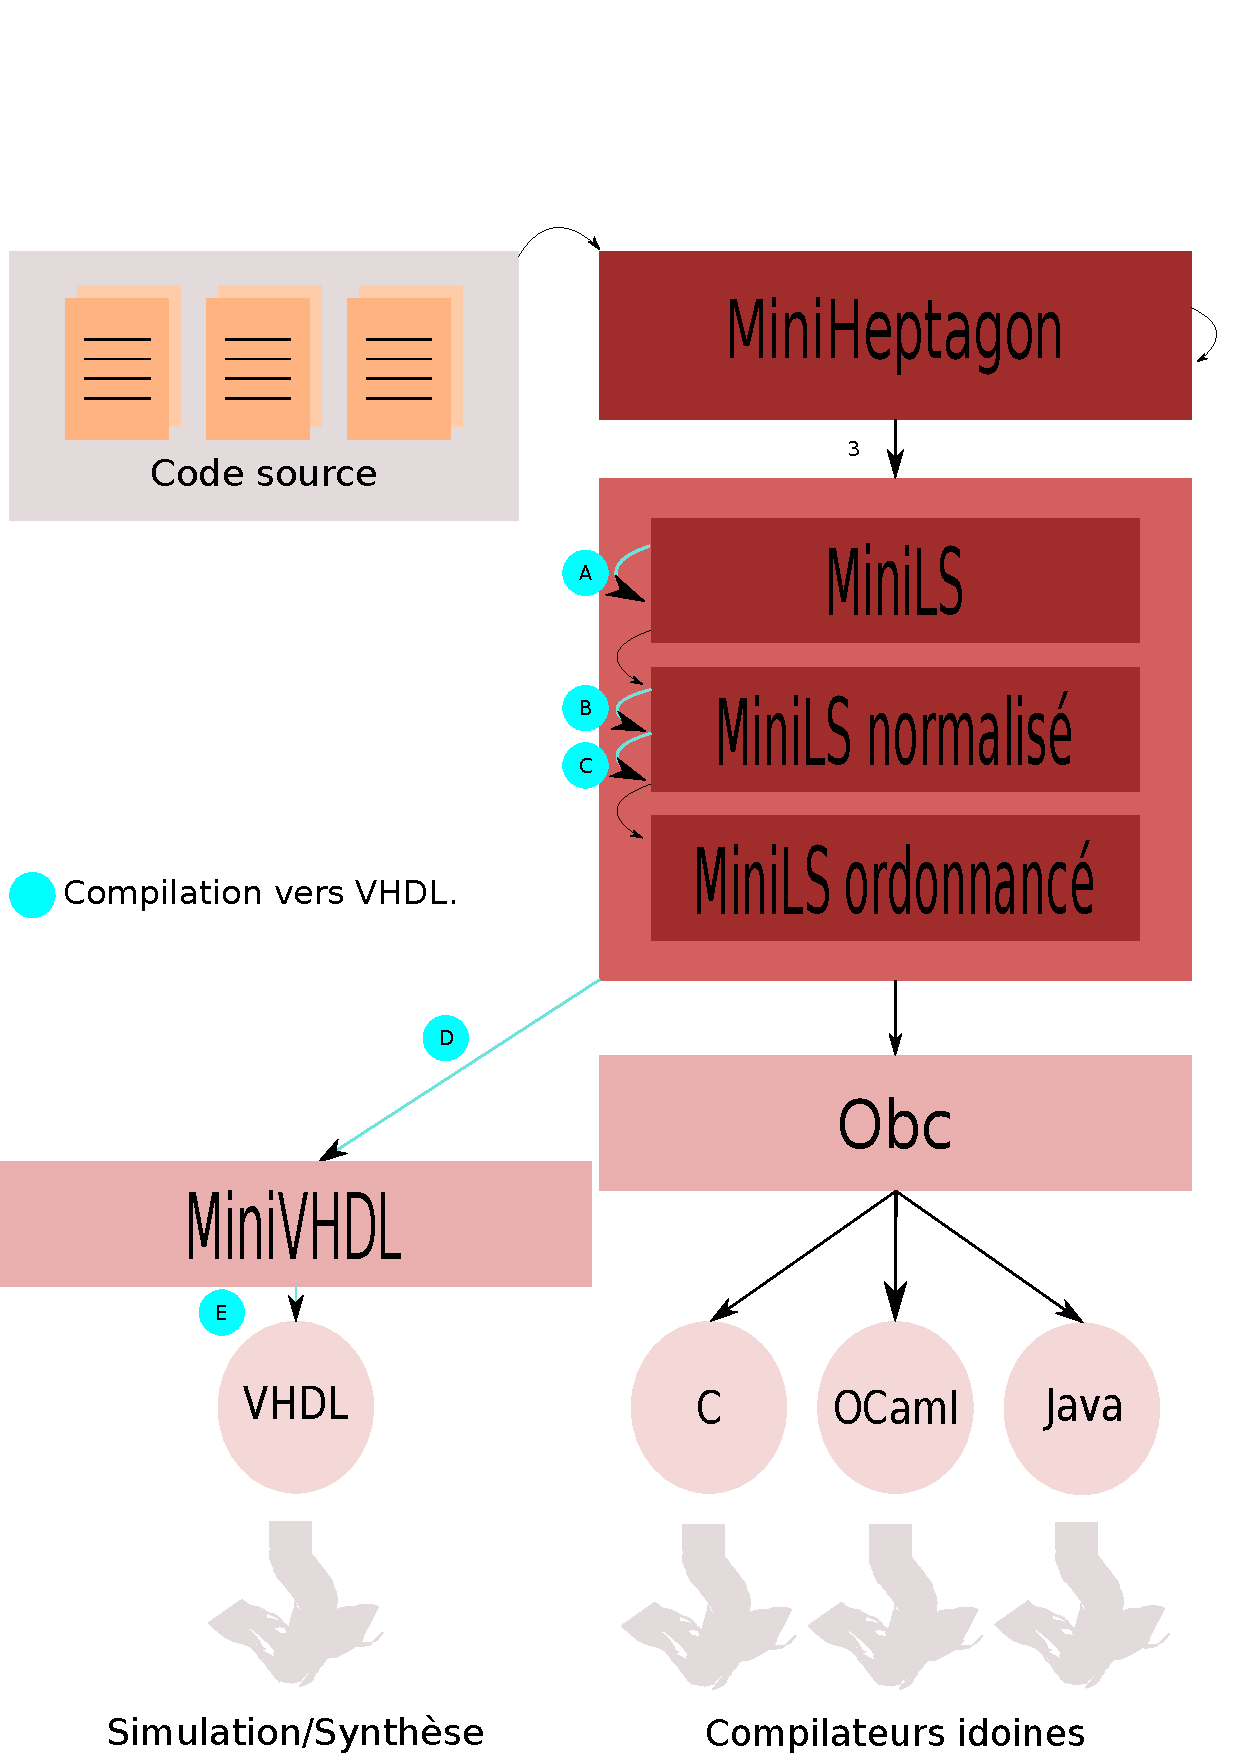
\includegraphics[scale=0.5]{archi}
  \caption{Architecture du compilateur \LANG{}}
  \label{fig:archi}
\end{figure}

Le passage au code séquentiel est court-circuité lors d'une compilation vers
VHDL, qui traduit MiniLS directement vers celui-ci. Pour faciliter cette étape,
on pratiquera en amont trois transformations simplificatrices sur MiniLS.

\renewcommand{\labelenumi}{\Alph{enumi}}
\begin{enumerate}
\item Suppression de la réinitialisation logique.
\item Suppression des itérateurs sur tableaux via mise à plat.
\item Introduction d'une variable intermédiaire pour chaque argument d'un appel
  de noeud.
\item Traduction vers un sous ensemble de VHDL baptisé MiniVHDL.
\end{enumerate}

Le code MiniVHDL obtenu peut ensuite être traité par les outil dédiés.

\section{De \LANG{} à VHDL}

\subsubsection{Syntaxes}

\TODO{Donner la forme originale sans reset telle qu'avant normalisation ?}

\paragraph{MiniLS}
\label{sec:syn:mls}

\begin{figure}[h]
  \centering
  \begin{eqnarray*}
    td & \Coloneqq & \mybox{type } bt = C + \dots + C \\
    d & \Coloneqq & \Node{p}{p}{p}{D} \\
    p & \Coloneqq & x : bt; \dots; x : bt \\
    D & \Coloneqq & pat = e; \dots; pat = e \\
    pat & \Coloneqq & x \p (pat,\dots,pat) \\
    e & \Coloneqq & x \p v \p \Op{e}{e} \p \Fby{v}{e} \p \Pre{e} \\
    & \p & \Every{f}{e}{e}{x} \p \When{e}{C}{x} \\
    & \p & \Merge{x}{C}{e}{C}{e} \\
    & \p & \Map{f}{e_1}{e_n} \\
    & \p & \Fold{f}{e_1}{e_n} \\
    & \p & \Mapfold{f}{e_1}{e_n} \\
    v & \Coloneqq & i \p C \\
    ck & \Coloneqq & \Base \p \On{ck}{C}{x}
  \end{eqnarray*}
  \caption{MiniLS}
  \label{fig:mls}
\end{figure}

MiniLS est équivalent au langage synchrone à flots de données bien connu qu'est
Lustre \cite{lustre}, auquel on adjoint une construction de réinitialisation
modulaire d'un noeud\footnote{$\Every{f}{e_1}{e_n}{z}$ appelle le noeud $f$ avec
  les arguments $e_1,\dots,e_n$, et réinitialise la mémoire de celui-ci lorsque
  $z$ est vraie.}.

Les programmes MiniLS sont présents dans le compilateur sous trois formes
distinctes ; la première est donnée par souci de cohérence et ne nous intéresse
pas directement, les précédentes passes du compilateur nous fournissant
directement la deuxième. Ce processus de compilation est décrit en détails dans
l'article \cite{lctes08a}.

\begin{itemize}
\item Forme originale \ref{fig:mls} telle qu'obtenue à partir du code \LANG{}
  original.
\item Forme normale \ref{fig:mlsn}.
\item Forme finale \ref{fig:mlsns}, normalisée, sans réinitialisations ($every$)
  ni itérateurs, et où tous les paramètres effectifs sont des noms
  d'identifiants.
\end{itemize}

On va décrire les constructions du langage :

\begin{figure}[htp]
  \centering
  \begin{eqnarray*}
    e & \Coloneqq & x \p v \p \Op{e}{e} \p \When{e}{C}{x} \\
    ce & \Coloneqq & e \p \Merge{x}{C}{ce}{C}{ce} \\
    eq & \Coloneqq & x = ce \p x = \Fby{v}{e} \p x = \Pre{e} \\
    & \p & (x,\dots,x) = \Every{f}{e}{e}{x} \\
    & \p & (x,\dots,x) = \App{f}{e,\dots,e} \\
    & \p & \Map{f}{e_1}{e_n} \\
    & \p & \Fold{f}{e_1}{e_n} \\
    & \p & \Mapfold{f}{e_1}{e_n}
  \end{eqnarray*}
  \caption{MiniLS normalisé}
  \label{fig:mlsn}
\end{figure}

\begin{figure}[htp]
  \centering
  \begin{eqnarray*}
    e & \Coloneqq & x \p v \p \Op{e}{e} \p \When{e}{C}{x} \\
    ce & \Coloneqq & e \p \Merge{x}{C}{ce}{C}{ce} \\
    eq & \Coloneqq & x = \Pre{e} \\
    & \p & (x,\dots,x) = \App{f}{x,\dots,x}
  \end{eqnarray*}
  \caption{MiniLS simplifié (et normalisé)}
  \label{fig:mlsns}
\end{figure}

\paragraph{MiniVHDL}

MiniVHDL \ref{fig:mvhdl} est un fragment très restreint de VHDL, suffisant pour
décrire l'essence de notre processus de traduction. Un composant MiniVHDL
$\Component{f}{P}{sigs}{lvars}{ports}{I}$ correspondra concrètement à un
composant VHDL formé des instantiations $ports$, signaux internes $sigs$ et d'un
processus avec les variables locales $lvars$ et de corps $I$.

Notons que les paramètres effectifs des instantiations de composants sont des
noms de signaux ; cela justifie la forme simplifiée MiniLS décrite au paragraphe
précédent.

\begin{figure}[htp]
  \centering
  \begin{eqnarray*}
    component & \Coloneqq & \mybox{component} \; f \; \mybox{port} \; sm;\dots;\
    sm \; \mybox{with} \, \mybox{sig} \; d; \dots; d \; \\
    & & \mybox{and} \, \mybox{var} \; d; \dots; d \; \mybox{and} \
    \mybox{subcomponents} \; p; \dots; p \; \mybox{in} \; I \\
    sm & \Coloneqq & x : mode \ ty \\
    sd & \Coloneqq & x : mode \ ty \coloneqq e \\
    mode & \Coloneqq & \mybox{in} \p \mybox{out} \\
    d & \Coloneqq & x : ty \\
    p & \Coloneqq & \mybox{port map } x (bd;\dots;bd) \\
    bd & \Coloneqq & x \Rightarrow x \\
    I & \coloneqq & i; \dots; i \\
    i & \Coloneqq & \Assign{x}{e} \p \Affect{x}{e} \p \Case{e}{v}{I}{v}{I} \\
    e & \Coloneqq & id \; \vert \; v \; \vert \; \Op{e}{e} \\
    v & \Coloneqq & i \; \vert \; ' bitp ' \\
    bitp & \Coloneqq & bit \p bit \  bitp \\
    bit & \Coloneqq & \mathbf{0} \p \mathbf{1} \\
    bt & \Coloneqq & \mybox{natural} \p \mybox{std\_logic} \p \mybox{bit}
    \p \dots
  \end{eqnarray*}
  \caption{MiniVHDL}
  \label{fig:mvhdl}
\end{figure}

% On y ajoute comme raccourci syntaxique l'instruction suivante : $$\mybox{if } e
% \mybox{ then } I \mybox{ else } J \equiv \mybox{case } e \mybox{ of } ('1'
% \Rightarrow I) ('0' \Rightarrow J)$$

\subsubsection{Simplification de MiniLS normalisé}

Nous effectuons donc trois passes pour simplifier le code MiniLS.

\paragraph{Élimination de la réinitialisation logique}

Certaines constructions de MiniLS proposent au programmeur une forme de
réinitialisation modulaire : les équations de la forme $\Fby{v}{e}$ d'un noeud
$f$ instancié par la construction $\Every{f}{e_1}{e_n}{z}$ doivent-être
réinitialisées dès lors que $z$ est vrai.

La première passe de simplification, qui s'exécute sur le code MiniLS obtenu à
la troisième étape du processus décrit plus haut, permet d'éliminer ces
constructions $every$ dans le but de compiler plus uniformément vers VHDL,
autrement dit sans nécessiter un traitement ad-hoc de la réinitialisation.

L'idée est d'ajouter à chaque noeud un argument supplémentaire nommé
\texttt{rst} correspondant à un appel nécessitant une réinitialisation de la
mémoire\footnote{On suppose évidemment que le nom \texttt{rst} est frais}. La
passe se charge de modifier les appels de noeuds pour synthétiser l'expression
correcte, en particulier dans le cas d'une équation de type $(x_1, \dots, x_n) =
\Every{f}{e}{e}{x}$ où $x$ doit être capable de réinitialiser $f$. Les mémoires
réinitialisables $\Fby{v}{e}$ doivent bien-entendu être réinitialisées lorsque
l'argument \texttt{rst} est vrai ; pour cela, il suffit de remplacer ces
dernières par $\If{rst}{v}{\newline \Pre{e}}$.

Les fonctions suivantes effectuent ces deux tâches : $RstE$ traite une
expression MiniLS, et $RstNode$ ajoute l'argument \texttt{rst} à un noeud et
transforme ses équations.

\newcommand{\re}[1]{RstE(#1)}
\newcommand{\rstn}[1]{RstNode(#1)}

\[
\begin{array}{lcl}
  \re{\Op{e_1}{e_n}} & = & \Op{\re{e_1}}{\re{e_n}} \\
  \re{\Fby{v}{e}} & = & \If{rst}{v}{\Fby{v}{\re{e}}} \\
  \re{\Pre{e}} & = & \Pre{\re{e}} \\
  \re{\Every{f}{e_1}{e_n}{x}} & = & \App{f}{\mathtt{rst} \; \mathbf{or} \;
    x, \re{e_1} \dots, \re{e_n}} \\
  \re{\App{f}{e_1,\dots,e_n}} & = &
  \App{f}{\mathtt{rst},\re{e_1},\dots,\re{e_n}} \\
  \re{\If{e_1}{e_2}{e_3}} & = & \If{\re{e_1}}{\re{e_2}\\ & & \hspace{1.7cm}}
  {\re{e_3}} \\
  \re{\When{e}{C}{x}} & = & \When{\re{e}}{C}{x} \\
  \re{\Merge{e}{C_1}{e_1}{C_n}{e_n}} & = &
  \mybox{merge} \; \re{e} \; (C_1 \Rightarrow \re{e_1}) \\
  & & \hspace{2.2cm} \dots \\
  & & \hspace{2.2cm} (C_n \Rightarrow \re{e_n})
\end{array}
\]

\[
\begin{array}{ll}
  RstEqs(pat_1 = e_1;\dots;pat_n = e_n) & = \\
  \ind pat_1 = \re{e_1};\dots;pat_n = \re{e_n} \\
  \rstn{\Node{f}{x_1,\dots,x_n}{y_1,\dots,y_n}{eqs}} & = \\
  \ind \Node{f}{rst,x_1,\dots,x_n}{y_1,\dots,y_n}{ResetEqs(eqs)}
\end{array}
\]

\paragraph{Suppression des itérateurs}

La version actuelle du compilateur et de son générateur de code VHDL supporte
les tableaux de dimension arbitraire \footnote{En pratique, les outils de
  synthèse de circuits à partir de code VHDL imposent une dimension maximale.}
et constructions associées ; il nous faut donc compiler les itérateurs
\texttt{map}, \texttt{fold} et \texttt{mapfold} vers VHDL.

Par souci de simplicité et uniformité, nous avons fait le choix de les éliminer
par \textit{inlining} lors d'une transformation source-à-source sur MiniLS. On
ne détaillera pas cette opération qui consiste simplement à remplacer les
itérateurs par plusieurs équations. L'équation $x = \Map{f}{t_1}{t_m}$ lorsque
les tableaux $t_1, \dots, t_m$ sont de taille $n$ sera ainsi remplacée par $n +
1$ équations dont les $n$ premières effectuent l'application de $f$ pour chaque
indice et la dernière affecte à $x$ le tableau en résultant. On applique des
transformations similaires aux opérateurs \texttt{fold} et \texttt{mapfold}.

\begin{figure}[htp]
  \centering
  \input{fold_orig}
  \caption{Calcul d'un ET logique via itérateur \texttt{fold}.}
  \label{fig:fold_orig}
\end{figure}

\begin{figure}[htp]
  \centering
  \input{fold_il}
  \caption{Calcul d'un ET logique, \texttt{fold} mis à plat.}
  \label{fig:fold_il}
\end{figure}

Le programme \ref{fig:fold_orig} présente un exemple effectuant un ET logique
sur tous les éléments d'un tableau via l'itérateur \texttt{fold}. Son pendant
avec itérateur mis à plat se contente de passer l'accumulateur d'élément en
élément \ref{fig:fold_il}.

\paragraph{Simplification des appels}

Comme nous le verrons plus bas, les appels de nœuds seront compilés en
instantiations de composants ; or, les arguments d'une construction VHDL $port
\; map$ sont forcément des identifiants. Autant se simplifier la tâche en amont
: on va donc transformer tout appel de noeud en introduisant une variable
intermédiaire pour chaque argument.

\newcommand{\simpl}[2]{Simpl(#1,#2)}
\newcommand{\simplnd}[1]{SimplNode(#1)}

\[
\begin{array}{ll}
  \simpl{x = ce}{eqs} & = \\
  \ind (x = ce) \Cons eqs \\
  \simpl{x = \Pre{e}}{eqs} & = \\
  \ind (x = \Pre{e}) \Cons eqs \\

  \simpl{(x_1,\dots,x_n) = \App{f}{e_1,\dots,e_n}}{eqs} & = \\
  \ind (y_1 = e_1) \Cons \dots \Cons (y_n = e_n)
  \Cons ((x_1,\dots,x_n) = \App{f}{rst,y_1,\dots,y_n}) \Cons eqs \\
  \ind \mbox{où } y_1,\dots,y_n \mbox{ sont des noms de variables frais}
\end{array}
\]

\[
\begin{array}{ll}
  \simplnd{\Node{x_1,\dots,x_n}{y_1,\dots,y_n}{p}{D}} & = \\
  \ind \mathtt{node} f(x_1,\dots,x_n) = y_1, \dots, y_n \; \\
  \ind \mathtt{with} \  \mathtt{var} \; p' \; \mathtt{in} \; fold\_right \; Simpl
  \; D \; [] \\
  \ind \mbox{en supposant que que } p' \mbox{ correspond} \\
  \ind \mbox{aux variables définies par les nouvelles équations.}
\end{array}
\]

Ces simplifications effectuées, on va s'atteler à la traduction de MiniLS vers
MiniVHDL.

\subsubsection{MiniLS simplifé vers MiniVHDL}

Les idées générales de la traduction de MiniLS simplifié vers MiniVHDL sont les
suivantes :

\begin{itemize}
\item Chaque noeud MiniLS correspondra à un composant (Mini)VHDL.
\item Chaque équation à mémoire (i.e. contenant $fby$ ou $pre$) va correspondre
  à un signal, chaque équation combinatoire à une variable locale.
\item La réinitialisation logique est gérée en amont comme expliquée ci-dessus,
  elle est donc implicitement asynchrone (indépendante des fronts montants de
  l'horloge).
\item Les partenaires ont exprimé le désir de pouvoir réinitialiser physiquement
  toute la mémoire lors du bascument d'un signal précis nommé
  \textbf{hwrst}\footnote{Le nom symbolique \textbf{hwrst} est supposé frais.} : on ajoute donc ce signal
  supplémentaire invisible dans le code MiniLS et on génère le code de
  réinitialisation correspondant lors du traitement du $fby$.
\item Pour respecter la sémantique à $\Delta$-cycles de VHDL, il importe de
  faire évoluer la mémoire par un pas du calcul uniquement sur front montant de
  l'horloge.
\item En suivant le modèle synchrone, les valeurs calculées par le circuit à
  d'autres moments que le front montant n'ont pas de sens bien défini ; on les
  ignorera donc.
\item Chaque appel de noeud correspondra à une instantiation. Comme spécifié
  plus haut, les paramètres effectifs d'un signal VHDL sont obligatoirement des
  signaux auxquels il faudra assigner la valeur correcte.
\end{itemize}

\paragraph{Traduction des types}

Les déclarations de types de données ont été laissées implicites aussi bien dans
la syntaxe de MiniLS que de MiniVHDL ; les possibilités étant exactement les
mêmes (énumérations et enregistrements), on choisit de ne pas s'attarder sur
leur traduction qui reste une traduction mot-à-mot d'une syntaxe concrète à
l'autre.

\paragraph{Traduction des constantes et fonction auxiliaires sur les horloges}

La fonction $TradConst$ traduit une constante MiniLS en constante MiniVHDL.

\newcommand{\TradC}[1]{TradConst(#1)}

\[
\begin{array}{lcl}
  \TradC{i} & = & i \\
  \TradC{true} & = & '1' \\
  \TradC{false} & = & '0' \\
  \TradC{C} & = & C
\end{array}
\]

La fonction auxiliaire $GuardClock$ permet de traduire une horloge MiniLS en
expression MiniVHDL de type booléen. Elle sera utilisée pour contrôler la mise à
jour des registres, s'assurant que cette dernière n'est effectuée qu'aux
instants où l'horloge est effective.

\newcommand{\GEC}[1]{GuardClock(#1)}

\[
\begin{array}{lcl}
  \GEC{\Base} & = & rising\_edge(clk) \\
  \GEC{\On{ck}{C}{x}} & = & x = \TradC{C} \; \mathtt{and} \; \GEC{ck}
\end{array}
\]

Tout comme les mises à jour des mémoires, les appels à d'autres noeuds sont
dirigés par les horloges qui en donnent la cadence. Il nous faudra donc une
fonction voisine de $GuardClock$ pour calculer l'expression MiniVHDL
correspondant à l'horloge utilisée dans l'appel d'un noeud.

\newcommand{\EC}[1]{ExpClock(#1)}

\[
\begin{array}{lcl}
  \EC{\Base} & = & clk \\
  \EC{\On{ck}{C}{x}} & = & x = \TradC{C} \; \mathtt{and} \; \EC{ck}
\end{array}
\]

\paragraph{Traduction des expressions et équations}

La fonction $TradExp$ traduit les expressions simples MiniLS normalisés et
simplifié en expressions MiniVHDL.

\newcommand{\TradE}[1]{TradExp(#1)}

\[
\begin{array}{lcl}
  \TradE{v} & = & \TradC{v} \\
  \TradE{x} & = & x \\
  \TradE{\Op{e_1}{e_n}} & = & \Op{\TradE{e_1}}{\TradE{e_n}} \\
  \TradE{\When{e}{C}{x}} & = & \TradE{e}
\end{array}
\]

La fonction $TradCExp$ traduit les expressions de contrôle formées d'expressions
simples ou de \texttt{merge} imbriqués en instructions MiniVHDL.

\newcommand{\TradCE}[2]{TradCExp(#1, #2)}

\[
\begin{array}{ll}
  \TradCE{x}{\Merge{y}{C_1}{ce_1}{C_n}{ce_n}} & = \\
  \ind \mathtt{case} \; y \; \mathtt{of} \;
  (\TradC{C_1} \Rightarrow \TradCE{x}{ce_1}) \\
  \hspace{2.1cm} \dots \\
  \hspace{2.1cm} (\TradC{C_n} \Rightarrow \TradCE{x}{ce_n}) \\
  \TradCE{x}{e} & = \\
  \ind \Affect{x}{\TradE{e}}
\end{array}
\]

Enfin, la fonction $TradEq$ permet de passer des équations aux instructions
MiniVHDL. Elle prend un argument supplémentaire permettant de compter le nombre
d'appels de noeuds afin de générer des arguments supplémentaires, et on se donne
une fonction supplémentaire $MakeArg(x,i)$ qui génère un nom de variable frais à
partir du nom de variable $x$ et de l'entier $i$.

La traduction des équations appelant un noeud nécessite des explications
concernant la façon de compiler les appels d'un noeud MiniLS qui seront données
à la section suivante.

\newcommand{\TradEq}[2]{TradEq(#1,#2)}
\newcommand{\MA}[2]{MakeArg(#1,#2)}

\[
\begin{array}{lcl}
  \TradEq{x = ce}{i} & = & \TradCE{x}{ce}, i \\

  \TradEq{x = \Pre{e}}{i} & = & \mathtt{if} \; \GEC{ck} \; \mathtt{then} \\
  & & \ind \Assign{x}{\TradE{e}} \\
  & & \mathtt{end} \; \mathtt{if}, i \\

  \TradEq{x = \Fby{y}{e}}{i} & = & \mathtt{if} \; \mathbf{hwrst}
  \; \mathtt{then} \\
  & & \ind \Assign{x}{y} \\
  & & \mathtt{elsif} \; \GEC{ck} \; \mathtt{then} \\
  & & \ind \Assign{x}{\TradE{e}} \\
  & & \mathtt{end} \; \mathtt{if}, i \\


  \TradEq{(x_1,\dots,x_n) = \App{f}{y_1,\dots,y_n}}{n} & = &
  \Assign{\MA{"ck"}{i}}{\EC{ck}} \\
  & & \Assign{\MA{y_1}{i}}{y_1} \\
  & & \dots \\
  & & \Assign{\MA{y_n}{i}}{y_n}, i + 1 \\
\end{array}
\]

Précisons que par construction, l'interface d'un composant est toujours de la
forme $(clk, in_1, \dots,in_n, out_1,\dots,out_n)$.

\paragraph{Gestion des tableaux}

Hormis le cas des itérateurs traités précédemment, la gestion des tableaux
n'appelle pas de commentaire particulier, à l'exception de l'anecdotique mais
gênante nécessité de déclarer à l'avance les types tableaux (bornes exclues) en
VHDL. Deux solutions sont envisageables :

\begin{itemize}
\item Calculer la dimension maximale des tableaux rencontrés dans le programme,
  et utiliser cette information pour pré-déclarer les tableaux VHDL idoines.
\item Déclarer quoi qu'il advienne les types de tableaux utiles et refuser les
  programmes comprenant des dimensions supérieures à une limite fixée à l'avance
  .
\end{itemize}

Le compilateur emploie pour l'instant la première méthode, mais la seconde ne
nous semble pas dérangeante pour des raisons pragmatiques\footnote{Notons que
  notre version de l'outil Xilinx ISE refuse par exemple tout tableau de
  dimension supérieure à trois.}.

\paragraph{Compilation modulaire et appels de noeuds}

MiniVHDL offre une forme de modularité basée sur une hiérarchie de
composants. Chacun de ces derniers spécifie une liste de composants fils dont
les ports (au sens de la figure \ref{fig:mvhdl}) sont instanciés avec des
signaux. Nous prenons donc soin d'utiliser des signaux comme résultats mais
aussi arguments ; par souci de simplicité, on introduit des signaux locaux pour
chaque argument, signaux qui seront affectés lors de la traduction de l'équation
correspondant à l'appel de noeud original.

La fonction $GatherPortMaps(D, i)$ rassemble cette liste de sous-noeuds à partir
des appels de noeud présents dans le paquet d'équations $D$ et créé les
instantiations de composants correspondantes. L'entier $i$ nous servira à
distinguer les appels de noeuds et de créer de nouveaux noms de signaux frais
grâce à la fonction $MakeArg$ décrite plus haut. On se donne également une
fonction $GetArgName(f,n)$ qui renvoie le nom du $n$-ème argument du noeud de
nom $f$.

\newcommand{\GPM}[2]{GatherPortMaps(#1,#2)}
\newcommand{\GAN}[2]{GetArgName(#1,#2)}

\[
\begin{array}{lcl}
  \GPM{[]}{i} & = & [] \\
  \GPM{((x_1,\dots,x_n) = \App{f}{y_1,\dots,y_n}) \Cons eqs}{i} & = &
  \\
  \ind \mybox{port map} \; f ( clk \Rightarrow \MA{"clk"}{i} \\
  \ind \ind \ind \ind \hspace{0.4cm} \GAN{f}{1} \Rightarrow \MA{y_1}{i} \\
  \ind \ind \ind \ind \hspace{0.4cm} \dots \\
  \ind \ind \ind \ind \hspace{0.4cm} \GAN{f}{n} \Rightarrow \MA{y_n}{i}) \\
  \ind \Cons \GPM{eqs}{i + 1}
\end{array}
\]

On définit ensuite les fonctions auxiliaires $NeedVar$, $Vars$, $ParamSigs$ et
$SignalOfVarDec$ respectivement chargées de déterminer si une équation introduit
des déclarations de variables locales ou non, de calculer la liste des variables
définies par une équation, de calculer les signaux à passer en arguments aux
appels de noeuds présents dans un paquet d'équations et enfin de traduire
simplement une déclaration de variable MiniLS en déclaration de signal MiniVHDL
avec mode d'utilisation (entrée ou sortie).

\newcommand{\NV}[1]{NeedVar(#1)}
\newcommand{\V}[1]{Vars(#1)}
\newcommand{\PS}[2]{ParamSigs(#1,#2)}
\newcommand{\SoVD}[3]{SignalOfVarDec(#1 : #2, #3)}

\[
\begin{array}{lcl}
  \NV{x = \Fby{v}{e}} & = & false \\
  \NV{(x_1,\dots,x_n) = \App{f}{y_1,\dots,y_n}} & = & false \\
  \NV{x = ce} & = & true
\end{array}
\]

\[
\begin{array}{lcl}
  \V{x = \Fby{v}{e}} & = & [x] \\
  \V{(x_1,\dots,x_n) = \App{f}{y_1,\dots,y_n}} & = & x_1 \Cons \dots \Cons x_n \\
  \V{x = ce} & = & [x]
\end{array}
\]

\[
\begin{array}{ll}
  \PS{x = \Fby{v}{e} \Cons eqs}{i} & = \PS{eqs}{i} \\
  \PS{(x_1,\dots,x_n) = \App{f}{y_1,\dots,y_n} \Cons eqs}{i} & = \\
  \ind \MA{"clk"}{i} \Cons \MA{y_1}{i} \Cons \dots \Cons \MA{y_n}{i} \\
  \ind \mathtt{::} \; \PS{eqs}{i + 1}
  \\
  \PS{x = ce \Cons eqs}{i} & = \PS{eqs}{i}
\end{array}
\]

\[
\begin{array}[lcl]{lcl}
  \SoVD{x}{bt}{mode} & = & \mybox{signal} \; x : mode \; TransBaseType(bt)
\end{array}
\]

\paragraph{Traduction des noeuds}

Enfin, $TradNode$ se charge de traduire un noeud en composant MiniVHDL, en
créant un signal local pour chaque équation retardée et argument d'appel de
noeud, une variable pour chaque équation combinatoire, et la liste de
sous-composants requise.

\begin{align*}
  & TradNode(\mybox{node } f(in) = out \mybox{ with var } p \mybox{ in } D) = \\
  & \bl \mbox{soit } port = \\
  & \bl \bl clk : \mybox{in std\_logic}; \\
  & \bl \bl \{ SignalOfVarDec(x : bt, \mybox{in}) \p (x : bt) \in in \}; \\
  & \bl \bl \{ SignalOfVarDec(x : bt, \mybox{out}) \p (x : bt) \in out \}, \\
  & \bl \mbox{ soit } signals = \{ \V{eq} \p eq \in D, \neg \NV{eq} \}
  \mybox{,} \\
  & \bl \mbox{ soit } sig\_args = \PS{D}{1} \mybox{,} \\
  & \bl \mbox{ soit } variables = \{ \V{eq} \p eq \in D, \NV{eq} \} \mybox{,} \\
  & \bl \mbox{ soit } ports = \GPM{D}{1} \mybox{,} \\
  & \bl \mbox{ soit } body = fold\_right TradEq D ([], 1) \mbox{ dans} \\
  & \mybox{component } f \mybox{ port } port \mybox{ with sig } signals \cup
  sig\_args \\
  & \mybox{and var } variables \mybox{ and subcomponents } ports \mybox{ in }
  body
\end{align*}

\section{Conclusion}

\TODO{À enrichir}

On a traduit \LANG{} vers VHDL en profitant des forces du modèle synchrone : sa
sémantique est bien adaptée à une description sous forme de circuits. Le
processus de traduction reste simple et compréhensible grâce aux garanties
offertes par le synchrone : nul besoin d'écrire plusieurs fois dans le même
élément mémorisant par cycle.

\appendix

\section{Exemples de code généré}

On présente ici quelques codes générés par notre prototype. En l'état actuel de
ce dernier, beaucoup de variables intermédiaires sont générées ; une passe
d'optimisation puissante est en développement.

On liste successivement le code MiniLS obtenu à partir de \LANG{}, puis le code
MiniLS normalisé et ordonnancé, et enfin le code VHDL.

\subsection{Compteur}

\paragraph{MiniLS initial}

\small
\input{compteur2_init}
\normalsize

\paragraph{MiniLS normalisé, ordonnancé et simplifié}

Notons que le noeud \textit{compteur} est ici instancié avec son paramètre
\textbf{n} égal à 4, ceci afin de pouvoir déplier les itérateurs.

\small
\input{compteur2_sched}
\normalsize

\paragraph{VHDL}

\small
\input{compteur2_vhdl}
\normalsize

\subsection{Allocateur de ressource}

\paragraph{MiniLS initial}

\small
\input{al2_init}
\normalsize

\paragraph{MiniLS normalisé, ordonnancé et simplifié}

\small
\input{al2_sched}
\normalsize

\paragraph{VHDL}

\small
\input{al2_vhdl}
\normalsize

\section{Utilisation du compilateur}

Nous supposerons dans ce manuel que l'archive du compilateur a été décompressée
dans le répertoire \verb/$HEPTDIR/. Cette archive contient le présent rapport,
un répertoire \texttt{exs/} avec une batterie d'exemples \LANG{} compilés vers
VHDL, et un binaire en code-octet pour la machine abstraite OCaml. Ce dernier
peut-être exécuté via \texttt{ocamlrun heptc}, ou bien directement lorsque votre
\texttt{ocamlrun} est présent dans \texttt{/usr/bin/}. Nous supposerons par la
suite que c'est le cas et que votre variable d'environnement \verb/$PATH/
contient \verb/$HEPTDIR/bin/.

Pour utiliser le compilateur, il faut tout d'abord renseigner la variable
d'environnement \verb/$HEPTLIB/ spécifiant au compilateur où trouver la
bibliothèque standard.

\begin{verbatim}
$ export HEPTLIB=$HEPTDIR/lib
\end{verbatim}

Vous pouvez ensuite vérifier que le compilateur est disponible et fonctionnel
via la commande suivante :

\begin{verbatim}
$ heptc -version
The Heptagon compiler, version 0.4 (wed. aug. 18 11:17:42 CET 2010)
Standard library in [...]
\end{verbatim}

Pour compiler un fichier \LANG{}, le compilateur doit être invoqué avec l'option
\verb/-target/. Les arguments possibles pour cette option sont :

\begin{itemize}
\item \verb/vhdl/ : génère du code VHDL.
\item \verb/mls/ : génère le code à flots de données MiniLS intermédiaire.
\item \verb/obc/ : génère un code impératif simple dans le langage idéalisé Obc.
\item \verb/c/ : génère du code C.
\end{itemize}

Les cibles VHDL et C invoquées sur un fichier \verb/source.ept/ produisent
respectivement un dossier \verb/source_vhdl/ et \verb/source_c/ qui contiennent
les fichiers sources générés. Par exemple :

\begin{verbatim}
$ cat source.ept
node main() returns (o : int)
let
  o = 0 fby (o + 1);
tel
$ heptc -target vhdl source.ept
$ ls source_vhdl
main.vhd  types.vhd
\end{verbatim}

L'option \verb/-s noeud/ permet de génèrer le code nécessaire à un exécutable
autonome à partir d'un fichier source \LANG{}, c'est à dire un
\textit{test-bench} dans le cas de VHDL et une fonction \verb/main()/ en ce qui
concerne C. Voici un exemple d'utilisation de la sortie C :

\begin{verbatim}
$ cat source.ept
node noeud() returns (o : int)
let
  o = 0 fby (o + 1);
tel

node main() returns (o : int)
let
  o = noeud() + 1;
tel
$ heptc -target c -s main source.ept
$ ls source_c
_main.c  _main.h  source.c  source.h  source_types.c  source_types.h
$ cc -Isource_c source_c/*.c -o source
$ ./source 5 # Option indiquant à l'exécutable généré de s'arrêter après 5 pas
=> 1
=> 2
=> 3
=> 4
=> 5
\end{verbatim}

\bibliography{biblio}
\bibliographystyle{plain}

\end{document}
